\subsection{Ejercicio 9}
  \begin{figure}
  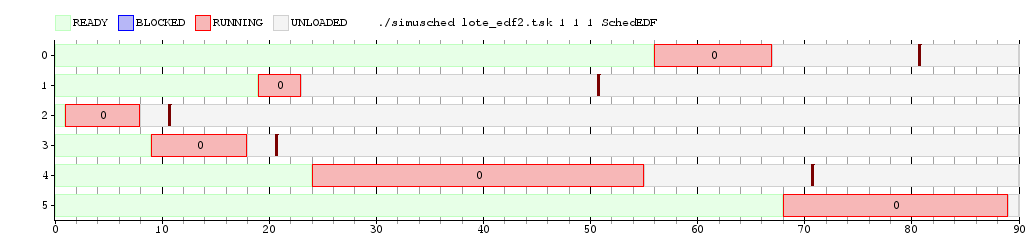
\includegraphics[scale=0.32]{images/lote2.png}
  \caption{Ejecuci\'on del scheduler EDF}
  \end{figure}
  \begin{figure}
  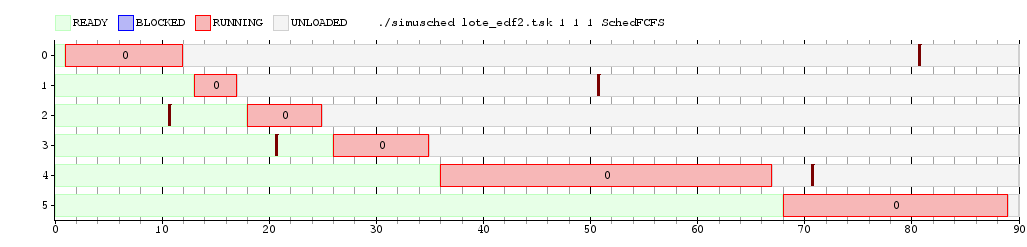
\includegraphics[scale=0.32]{images/lote2fcfs.png}
  \caption{Ejecuci\'on del scheduler FCFS}
  \end{figure}
  \begin{figure}
  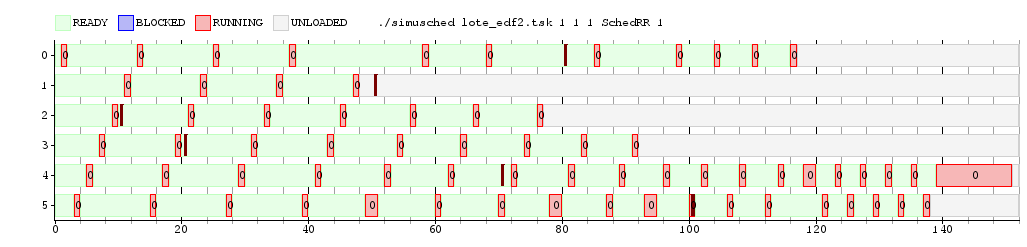
\includegraphics[scale=0.32]{images/lote2rr.png}
  \caption{Ejecuci\'on del scheduler Round Robin}
  \end{figure}
  \begin{figure}
  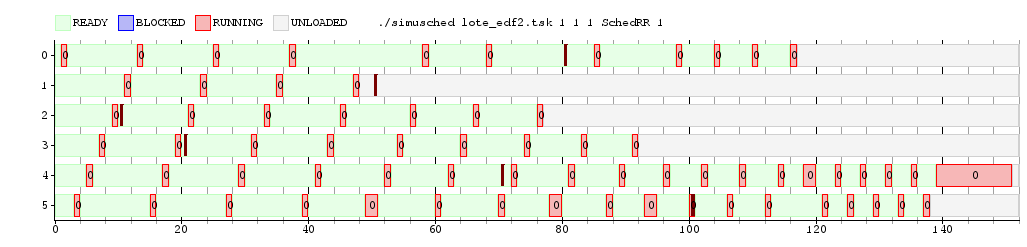
\includegraphics[scale=0.32]{images/lote2rr2.png}
  \caption{Ejecuci\'on del scheduler Round Robin 2}
  \end{figure}
Como se puede ver en los graficos de lote2 (figuras de 10 a 13), el unico scheduler que puede hacer que todas las tareas con deadline se realicen dentro de su limite es el EDF.
El scheduler EDF posee una propiedad que es condicion suficiente para asegurar esto, ademas de asegurar optimalidad.
Esta propiedad consiste en que si la sumatoria de la cantidad de ciclos de cada tarea divido su deadline es menor a 1, entonces el EDF va a encontrar una forma de ejecutar todas las tareas, y que además es óptima. Como se ve en los casos de las 2 implementaciones de round robin, y con el fcfs, todos fallan en lograr que todas las tareas se cumplan dentro de su deadline.
El FCFS falla al ir asignando las tareas como vienen, sin tener en cuenta nada más, por lo que al no priorizar las tareas con deadline próximos aunque hayan llegado ultimos, estos fallan.
El round robin no logra cumplir con los deadline debido a que su objetivo es tratar de balancear el uso de cpu por parte de tareas que tienen uso intesivo de cpu y tareas bloqueantes, de manera tal que no haya starvation de cpu para las tareas bloqueantes, y mientras estas estan bloqueadas, maximizar el uso de cpu, usando un quantum para mantener un balance entre las tareas. Este quantum evita que una tarea prioritaria con deadline proximo y un requirimiento de tiempo de cpu mayor a quantum se complete en el tiempo requerido.